\section{Compilation}
\label{sec:compilation}





\subsection{Overview}

\begin{figure}[t!]
\centering
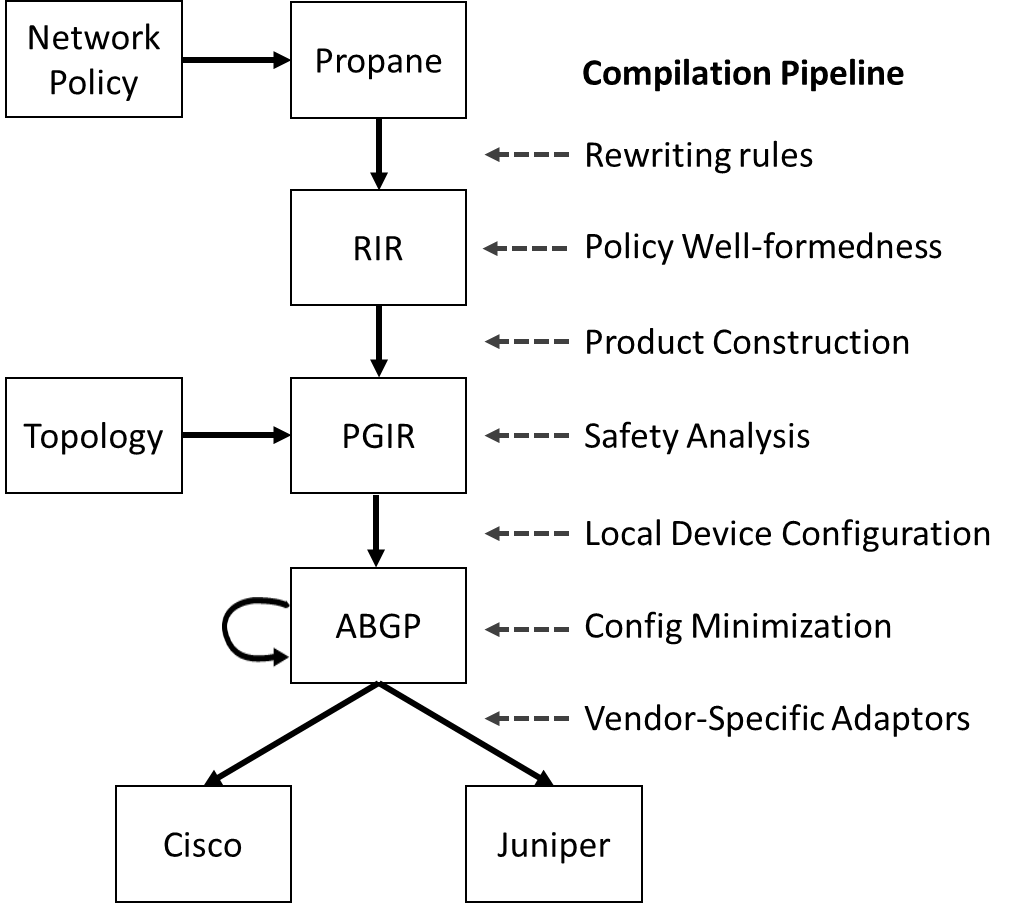
\includegraphics[width=\columnwidth]{figures/pipeline}
\caption{Compilation pipeline stages for Propane.}
\label{fig:pipeline}
\end{figure}

In this section we briefly describe our compilation strategy for \sysname. Figure~\ref{fig:pipeline} shows the 5 stage compilation pipeline to translate user-level \sysname policies into vendor-specific, device-local BGP policies. The first stage of the pipeline involves simple rewriting rules and substitutions from the user-level languae into the core Regular Intermediate Representation (RIR). Policies in RIR are checked for well-formedness (e.g., never constraining traffic that does not enter the network), before being combined with topological information to obtain Product Graph Intermediate Representation (PGIR). The PGIR is a data representation that compactly captures the control flow of all BGP advertisements subject to the policy and topology restrictions. We develop efficient algorithms that operate over the PGIR to ensure policy compliance, guarantee failure safety, avoid BGP instability, and prevent aggregation-induced black holes. Once the compiler determines the PGIR for the policy is safe, the compiler uses a simple translation to an abstract BGP (ABGP) representation. To make configurations more readable for human operators, and to reduce the size of the resulting configurations, the \sysname compiler makes several passes over ABGP form. Finally, vendor-specific adaptors can be added to \sysname to translate from ABGP to actual concrete configurations that go on the network devices.





\subsection{Regular IR (RIR)} 
\label{sec:rir}

The high-level language presented in Section~\ref{sec:propane} is just a thin layer on top of a core, regular-expression-based language for describing preference-based path constraints. Regular expressions are an expressive formalism that have been studied extensively for their ability utility in describing paths through graphs~\cite{bib:todo}, and applications to networks~\cite{bib:todo}. We present our core Regular language in the below.

% grammar
\newcommand{\BNFALT}{\;\;|\;\;}
\newcommand{\hdr}[2]{\flushleft \chdr{#1}{#2}}
\newcommand{\chdr}[2]{\textbf{#1} {#2} \\ \centering}

\begin{figure*}
  \begin{minipage}[t]{.45\linewidth}
  \hdr{\large Syntax}{}
  \vspace*{-1\baselineskip}
  %
  \[ \begin{array}{rclr}
    \hline

     pol     &::=& p_1, \dots, p_n & \textit{constraints} \\
     p       &::=& t \mapsto r_1 \gg \dots \gg r_m & \textit{preferences} \\
     t       &::=& & \textit{test} \\
         &\BNFALT& true & \textit{true} \\
         &\BNFALT& \neg t & \textit{negation} \\
         &\BNFALT& t_1 \vee t_2 & \textit{disjunction} \\
         &\BNFALT& t_1 \wedge t_2 & \textit{conjunction} \\
         &\BNFALT& prefix = x & \textit{prefix test} \\
         &\BNFALT& comm = c & \textit{community test} \\
     r       &::=& & \textit{regular paths} \\ 
         &\BNFALT& n & \textit{AS number} \\
         &\BNFALT& in & \textit{internal loc} \\
         &\BNFALT& out & \textit{external loc} \\
         &\BNFALT& r_1 \cup r_2 & \textit{union} \\
         &\BNFALT& r_1 \cap r_2 & \textit{intersection} \\
         &\BNFALT& r_1 \cdot r_2 & \textit{concatenation} \\
         &\BNFALT& !(r) & \textit{path negation} \\
         &\BNFALT& r^* & \textit{repetition} \\
     l       &::=& r_1 \rightarrow r_2 & \textit{link pairs} \\
     cc     &::=& agg(x, l) \BNFALT tag(c, t, l) & \textit{control constraints} \\
  \end{array} \]

  \end{minipage}
  %
  ~~
  \vrule
  ~~
  %
  \begin{minipage}[t]{.5\linewidth}
  \hdr{\large Propane Expansions}{}
  \vspace*{-1\baselineskip}
  %
  \[ \begin{array}{rcl}
    \hline
    any           & = & out^* \cdot in^+ \cdot out^* \\
    internal      & = & in^+ \\
    external      & = & out^+ \\
    only(X)       & = & any \cap X^* \\
    never(X)      & = & any \cap (!X)^* \\
    through(X)    & = & out^* \cdot in^* \cdot X \cdot in^* \cdot out^* \\
    after(X)      & = & out^* \cdot (X \cap out) \cdot out^* \cdot in^+ \cdot out^* \\
    before(X)     & = & out^* \cdot in^+ \cdot out^* \cdot (X \cap out) \cdot out^* \\
    end(X)        & = & any \cap (\Sigma^* \cdot X) \\
    start(X)      & = & any \cap (X \cdot \Sigma^*) \\
    exit(X)       & = & (out^* \cdot in^* \cdot (X \cap in) \cdot out \cdot out^*) \cup \\
                  &        & (out^* \cdot in^+ \cdot (X \cap out) \cdot out^*) \\
    enter(X)      & = & (out^* \cdot out \cdot (X \cap in) \cdot in^* \cdot out^*) \cup \\
                  &        & (out^* \cdot (X \cap out) \cdot in^+ \cdot out^*) \\
    link(X,Y)     & = & any \cap (\Sigma^* \cdot X \cdot Y \cdot \Sigma^*) \\
    path(\vec{X}) & = & any \cap (\Sigma^* \cdot X_1 \dots X_n \cdot \Sigma^*) \\
    novalley(\vec{X}) & = & any ~ \cap \\
                  &   & !path(X_2,X_1,X_2) ~ \cap \dots \cap \\ 
                  &   & !path(X_n,X_{n-1},X_n) \\
  \end{array} \]

  \end{minipage}

  \hrulefill

  \caption{Regular Intemediate Language (RIL) syntax (left), and 
           Propane language expansions (right).}
  \label{fig:rir-syntax}
\end{figure*}


\para{Syntax}

The syntax for the RIR is shown in Figure~\ref{fig:rir-syntax}. A policy consists of one or more constraints, each of which consists of a test on the type of route, and a corresponding set of preferred regular paths. Regular paths are simply regular expressions where the base locations are AS numbers. Special \textit{in} and \textit{out} symbols are used to refer to any internal or external location respectively.
For example, the constraint 
$$prefix=74.125.28.0/24 \mapsto (200 \cdot in \cdot in^*) \gg (100 \cdot in \cdot in^*)$$
describes a more-preferred set of paths for traffic announced by a prefixes no less specific than $74.125.28.0/24$, which starts at AS 200, before entering and staying inside the user's network to get to the destination, and a less-preferred set of paths that start at AS 100 and are otherwise the same. Tests over route types are allowed to be used with standard boolean connectives, and they can refer to both prefixes and community values (which are often important when interoperating with existing ASes).

\sysname also supports constraints purely on the control-plane behavior of the BGP routing protocol. Thing like prefix aggregation, which should not affect routing behavior, is an important optimization to reduce routing table size and churn. Aggregation, for example from internal locations and external locations, is specified using the same regular syntax as before: 
$$agg(128.17.0.0/16, in \rightarrow out)$$
where the expression $in \rightarrow out$ refers to control messages flowing from any internal location to any external location.

We list the route aggregation and community tagging constraints in Figure~\ref{fig:rir-syntax}, however our implementation also supports other constraints such as limiting the maximum number of routes, or enabling BGP multipath.


\para{Semantics}

The semantics of RIR can be thought of in terms of ranked paths. Each preference-based regular path constraint (of the form $r_1 \gg \dots \gg r_j$) maps to a set of concrete paths in the network that match one of $r_i$. We denote a network path as a string of ASes of the form: $n_1 n_2 \dots n_k$, and we say regular expression $r$ matches path $p$, if $p \in \mathcal{L}(r)$ and $p$ is a topologically-valid path. We denote the length of a path $p$ as $\abs{p}$. A path $p$ will have a rank: 
$$(\min_i \set{ p \in \mathcal{L}(r_i) }, \abs{p})$$
where the rank is lexicographically ordered according to (1) the most preferred regular expression matched, and (2) as a tie breaker, the length of the path. A lower rank indicates a \emph{more} preferred path. The desired semantics is to allow traffic to be sent along any of the most preferred paths for any pair of starting and ending locations that appear in some valid path. 

The set of ranked paths depends on which paths are valid given the topology, and thus when failures occur, so do the most preferred routes. It is the job of the \sysname compiler to ensure that generated configurations for a policy always achieve the most preferred path possible given the failures in the topology, and it must do so using purely distributed mechanisms.


\para{Propane to RIR}

The main differences between \sysname the regular language are: (1) \sysname allows the programmer to specify constraints separately, and combine them together modularly, (2) \sysname provides high-level names that abstract sets of routes, and (3) \sysname allows the preference operator to appear in more locations.
The translation from \sysname to RIR is based on a set of simple rewriting rules.

One of the main constraints when translating to RIR is to ensure that all specified routes are well-formed. In particular, each regular path constraint $r$ must satisfy $r \subseteq out^* \cdot in^+ \cdot out^*$. This ensures that one can only ever talk about controlling traffic that goes through the user's network at some point.

The first step is to merge separate constraints. This is accomplished by simply taking the cross product of per-prefix constraints, where logical conjunction ($a \wedge b$) is replaced by intersection on regular constraints ($a \cap b$), logical disjunction is replaced by union, and logical negation ($\neg a$) is replaced by ($any \cap !(a)$).
%
For example, in the data center configuration from Section~\ref{sec:propane}, combining the \textit{Routing} and \textit{Ownership} constraints would result in the following RIR configuration:

\begin{lstlisting}[mathescape=true]
$\path{p_{g1}}{any \cap end(A)}$
$\path{p_{g2}}{any \cap end(B)}$
$\path{p_{l1}}{\neg enter(out) \cap end(E)}$
$\path{p_{l2}}{\neg enter(out) \cap end(F)}$
$\path{true}{exit(out)}$
\end{lstlisting}

The next step is to rewrite the high-level constraints such as \textit{enter} and \textit{exit} according to the equivalences listed in Figure~\ref{fig:rir-syntax}. Since preferences can only occur at the top level for RIR, the final step is to lift the preferences that occur in the regular expression. For example, the regular expression $a \cdot (b \gg c) \cdot d$ is lifted to $(a \cdot b \cdot d) \gg (a \cdot c \cdot d)$. In general, we employ the follwing:
%
$$x \odot (y_1 \gg \dots \gg y_n) = x \odot y_1 \gg \dots \gg x \odot y_n$$
%
where $\odot$ stands for an arbitrary regular binary operator. Preferences nested under a unary operator, \textit{star} or \textit{negation}, are invalid policies.





\subsection{Product Graph IR}


\newcommand{\state}[4]{\node[state,#3](#1)[#4]{#2};}
\newcommand{\transition}[4]{\path[->] (#1) edge [#4] node {#3} (#2);} 


\begin{figure*}
  \begin{minipage}[t]{.5\linewidth}
  \hdr{\large Topology}{}
  \vspace*{-1\baselineskip}
  
  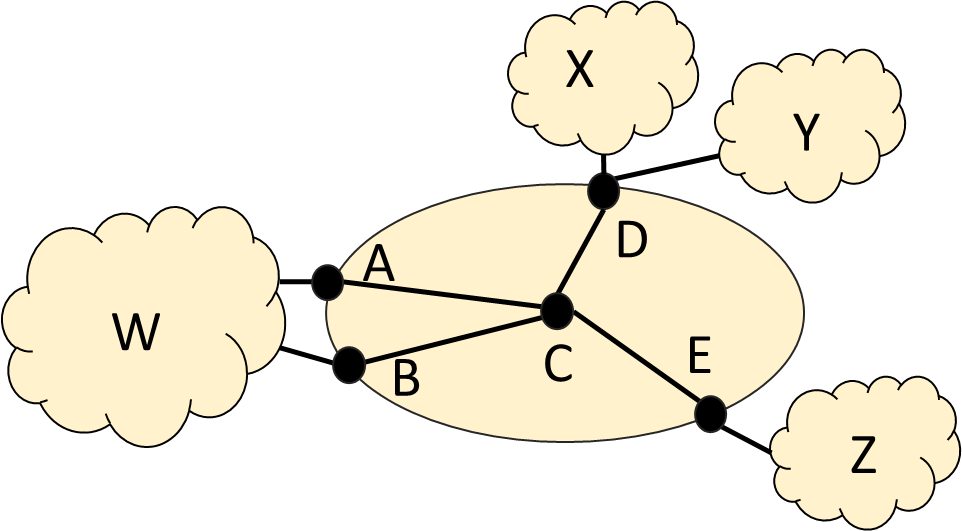
\includegraphics[width=.8\columnwidth]{figures/topology}
  
  \hdr{\large Policy Automata}{}
  \vspace*{1\baselineskip}
    
  \begin{tikzpicture}[>=stealth',shorten >=1pt,auto,node distance=1.6cm]
    \state{0}{$0$}{              }{}
    \state{1}{$1$}{right of=0}{}
    \state{2}{$2$}{right of=1}{}
    \state{3}{$3$}{right of=2}{}
    \state{4}{$4$}{right of=3}{}
    \state{5}{$5$}{right of=4}{accepting}
    \transition{0}{1}{out}{}
    \transition{1}{2}{D}{}
    \transition{2}{3}{C}{}
    \transition{3}{4}{A}{}
    \transition{4}{5}{W}{}
  \end{tikzpicture}
  
  \begin{tikzpicture}[>=stealth',shorten >=1pt,auto,node distance=1.6cm]
    \state{0}{$0$}{              }{}
    \state{1}{$1$}{right of=0}{}
    \state{2}{$2$}{right of=1}{}
    \state{3}{$3$}{right of=2}{}
    \state{4}{$4$}{right of=3}{accepting}
    \transition{0}{1}{out}{}
    \transition{1}{2}{in}{}
    \transition{2}{2}{ACDE}{loop above}
    \transition{2}{3}{B}{}
    \transition{3}{3}{B}{loop above}
    \transition{3}{2}{ACDE}{bend left}
    \transition{3}{4}{W}{}
  \end{tikzpicture}
   
  
  \end{minipage}
  %
  ~~
  ~~
  %
  \begin{minipage}[t]{.5\linewidth}
  \hdr{\large Product Graph}{}
  \vspace*{-1\baselineskip}
  %
  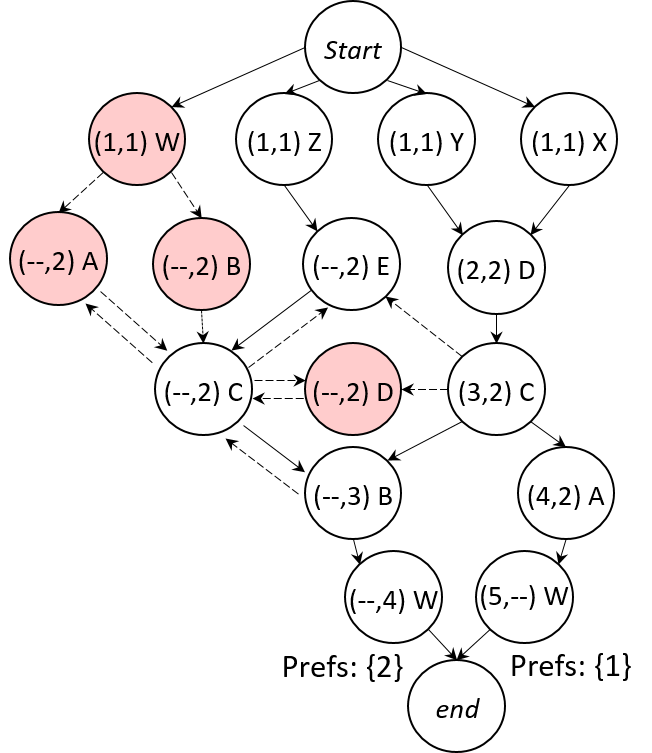
\includegraphics[width=.8\columnwidth]{figures/productgraph}
  \end{minipage}

  \hrulefill

  \caption{Example Product Graph construction.}
  \label{fig:example-compilation}
\end{figure*}


Now that the user policy exists in a simplified form, we must take the topology into consideration. In particular, we are interested in a compact representation that describes all the possible ways BGP route advertisements can flow through the network subject to the policy and topology constraints. To this end, we use a Product Graph Intermediate Representation (PGIR) to capture these dependencies. The Product graph can be thought of as the intersection of each of the regular automata corresponding to the RIR path preferences, and the topology. Finding paths through a graph subject to regular constraints has been studied extensively in the database literature~\ref{bib:todo}, and has been applied to networks in the past~\ref{bib:todo}.

\para{Formal definition}

The translated user policy into RIR is of the form $r_1 \gg \dots \gg r_j$. While paths talk about the direction traffic flows through the network, to implement the policy with BGP we are concerned about the way control-plane information is disseminated (i.e., router advertisements flowing in the opposite direction). To capture this idea, for each regular expression $r_i$, we construct a deterministic finite state machine on the reversed regular expression. Each automaton is a tuple: ($\Sigma, Q_i, F_i, q_{0_i}, \sigma_i$). The alphabet $\Sigma$ consists of all internal and external ASes, $Q_i$ is a set of states, $F_i$ is the set of final states, $q_{0_i}$ is the initial state, and $\sigma_i \colon Q_i \times \Sigma \rightarrow Q_i$ the state transition function.

The topology is modelled as a graph ($V, E$), which consists of a set of vertices $V$, and a set of directed edges $E \colon 2^{V \times V}$.

\todo{use different symbols here}

The combined product graph is a tuple: ($V'$, $E'$, $s$, $A$) with 
vertices $V' \colon V \times 2^{Q_1 \times \dots \times Q_j}$, 
edges $E' \colon 2^{V' \times V'}$, 
a unique starting vertex $s$, 
and an preference function $P \colon V \rightarrow 2^{\set{1, \dots, j}}$ , which maps nodes in the graph to the set preferences for which the corresponding automata are accepting in state $Q_i$


\para{From RIR To PGIR}

Intuitively product graph tracks which states of each automaton the policy is in as traffic moves between different topology locations. 

Consider the topology shown in Figure~\ref{fig:example-compilation}. Suppose we want to set up a primary route from W that enters the network from $A$, and utilizes the A -- C and C -- D links. We also would like a backup route that utilizes enters from node $B$, and utilizes the B -- C link, but is otherwise unconstrained. For the sake of simplicity, we will assume that the route can end in either $X$, $Y$, or $Z$. The RIR for the policy is:
%
$$(W \cdot A \cdot C \cdot D \cdot out) \gg (W \cdot B \cdot in^* \cdot out)$$
%
Figure~\ref{fig:example-compilation} shows the policy automata for each regular expression preference. Since we are interested in the flow of control messages, the automata match backwards. Figure~\ref{fig:example-compilation} shows the product graph obtained from intersecting the topology and policy automata. Every path in the product graph corresponds to a concrete path in the topology. In particular, every path through the product graph that ends at a node with an accepting preference is a valid topological path that satisfies the policy constraints and results in a particular preferenced path.
%
For example, the path $X D C A W$ is a valid path in the topology that BGP route advertisements might take, which would lead to obtaining the most prefered preference.
BGP control messages can start from peer X, which would match the $out$ transition from both automata, leading to state $1$ in the first automaton, and state $1$ in the second automaton. This is reflected in the product graph by the node with state $(1,1) X$. From here, if X were to advertise this route to D, it would result in the path $D X$, which would lead to state $2$ in the first automaton, and state $2$ in the second automaton, and so on. Since node $(5,-) W$ is in an accepting state for the first automata, it indicates this path has preference 1.

\todo{explain drop states}
\todo{preferences are reversed in picture}

\para{Minimization}

Although every path through the product graph is a valid path in the topology, we do not want to consider loops when configuring the network. In particular, BGP's loop prevention mechanism (where an AS rejects any route for which it is already in the AS path), means that loops should never occur.\footnote{Misconfigured aggregation can still lead to loops in BGP}
%
However, the product graph may contain many paths that form loops in the topology. For example, in Figure~\ref{fig:example-compilation}, the path $W A C B W$ is a valid path that BGP route advertisements might take through the topology, leading to a path that satisfies the preference 1 policy, but which contains a loop.
%
Since we are primarily concerned with guaranteeing user policy correctness and safety with respect to network failures, it is useful to avoid considering possibilities that are not possible due to loops. For example, if we can safely remove an edge from the product graph, then we don't have to consider the case that the edge has failed. 

We can safely remove any node or edge from the product graph so long as it never appears on any \emph{simple} path from the \textit{start} node to some node with an accepting preference. For example, node $(1,1) W$ in Figure~\ref{fig:example-compilation} is never on a simple path to an accepting preference since both end at location $W$.
%
Although fully minimizing the product graph is an NP-complete problem, we find that a simple and efficient algorithm based on graph dominators achieves largely the same effect, without preventing compilation of most policies in practice. 

A node $x$ dominates node $y$ if $x$ appears on every path leading to $y$ from the $start$ node. Many algorithms for finding graph dominators efficiently exist~\ref{bib:todo}. To minimize the product graph, we compute the dominator set for each node in both the product graph $G$, and the reversed product graph $G^R$ (with a source node attached to each accepting state). The following rules us to efficiently simplify the product graph.


\begin{itemize}
  \item Remove nodes that never reach an accepting state
  \item Remove nodes not reachable from the $start$ node
  \item Remove any node $x$ such that $x$ is dominated by $y$ in $G$ or $G^R$, and $loc(x) = loc(y)$
  \item Remove any edge from $x$ to $y$ in $G$ or $G^R$ if there is some $z$ dominated by $y$ such that $loc(x) = loc(z)$
\end{itemize}

Repeated application of the 4 above rules leads to removing the colored nodes and dashed lines in Figure~\ref{fig:example-compilation}. 

\para{Failure Safety}

To implement backups in routing, BGP uses local preferences on a per-device basis. However, the distributed nature of BGP makes setting preferences locally to achieve a network-route routing policy difficult, particularly in the presence of failures. For example, imagine an extremely simple policy for the topology in Figure~\ref{fig:example-compilation}, which says to prefer $WACD$ over $WBCE$:
%
$$(W \cdot A \cdot C \cdot D) \gg (W \cdot B \cdot C \cdot E)$$
%
How could such a policy be implemented in BGP? Suppose we simply set the local preference at router $C$ to prefer $D$ over $E$. However, now if the A -- C link fails, then suddenly $C$ has made the wrong decision and can not get either the primary or backup route specified, despite the fact that $W \cdot B \cdot C \cdot E$ route is available.

In particular, any time a router must make a decision locally between several route options, there is the possibility that it might choose incorrectly and regret its decision. The product graph representation captures this notion of choice precisely. For example, router $D$ in Figure~\ref{fig:example-compilation} appears only once in the product graph, possible receiving route advertisements from $Y$ or $X$. However, regardless of where 









\para{Notes}

\begin{itemize}
	\item Separate prefixes so they are disjoint
	
	\item For each prefix, build a DFA from each of the regular path constraints
		  We do this using character classes and regular expression derivatives.
		  The accepting states are labeled with the particular preference.
	
	\item Build the constraint graph, which gives us valid paths through the network that satisfy one or
		  more of the regular path constraints. We accept if we are in at least one of the accepting states
		  for one or more of the DFAs. Add a new start and end node as well.
		
	\item Minimize the constraint graph by removing nodes and edges that never contribute to a solution.
		  Required for soundness. Removing these makes it easier to check if things are implementable using BGP (see next point).
		  We use several heuristics to make this faster (e.g., removing edges for dominated nodes)
		
	\item Since our policy language can express things not implementable in BGP, we need a few checks.
		  First show some examples of what the problem is: why BGP cannot make a decision.
		  The reasons this can happen are:
		  (1) Single best path per router - no subset of paths specified is consistent (if A goes through B and C goes through A, then C goes through B).
		  (2) Failures - Have to make a decision without knowing what failures have occurred. Never want to prefer one peer over another and then not get a path when one was available

	\item We can check for these with a sufficient condition (that works often and is very fast),

	\item For each router, build a preference pre-order, that defines the constraints between preferences.
	
	\item Finally, if we know BGP can make decision locally, then we can directly translate to local BGP configurations using
		  information about the state machines from the neighbors. In particular, we tag (and test on) community values for the
		  corresponding state and set preferences accordingly (example will be needed)

	\item Running example will be helpful here.	
\end{itemize}


\subsection{Optimizations}

\begin{itemize}
	\item For performance, the main bottleneck will probably be the minimization step. We use a number of heuristics here to make this faster.
	\item For config readability and number of route maps/communities, we avoid community tagging/matching whenever possible with a number of tricks.
\end{itemize}



